\documentclass[a4]{article}
\usepackage{graphicx} 
\author{Group 7, System Black}
\title{Software Requirements Specification}

\begin{document}
\maketitle
\section{Introduction}
\subsection{System Name}
Score Management Subsystem of the Teaching Service System
\subsection{Overview}
Score management system is a critical component of teaching service system that provides support on score record, score query and score analysis. Up to now, we specified two major groups of actors as instructors and students and authorized them different accessibility to each function. We took use of the UML model include use case diagram, data flow diagram, state diagram, class diagram and CRC cards to elucidate our design. The details will be discussed in the following chapters.
\subsection{Developers}

Group-Black-7 is responsible for the Score Management Subsystem of the Teaching Service System. The members of the group are:

\begin{itemize}
\item Qi, ZHU

\item Shijia, WEI

\item Shiyi, ZHU

\item Tao, LIN

\item Ye, QI
\end{itemize}
(In Alphabetical Order)

\subsection{Background}
\subsubsection{Customer}
Yue Chen, faculty of CS Department, Zhejiang University 
\subsubsection{Latent User} 
Faculties, students, administrators and system maintainers of Zhejiang University
\subsubsection{Running Environment} 
Local Area Network of a university

\subsubsection{Purpose of this Document}
This document provides a specific rule of the development of Score Management Subsystem of the Teaching Service System. This document declare the specific role of each part in the subsystem.  The document is developed under the consensus of both customers and developers, which will eventually help two groups to build mutual understanding and better communication. 

And the specific purpose are:
\begin{itemize}
\item To provide a detailed document of what is to be developed.
\item To provide a detailed document of how the subsystem is developed.
\item To provide a detailed document of how inspection is conducted.
\end{itemize}
\subsubsection{Purpose of this Project}
The system aims to provide a service that helps the faculties and school administrators with the score management. The system provides integrity, usability and security of the service. As the system developers are university undergraduate students, the project also aims to develop students' capability of planning, designing, implementing, testing, documenting and teamwork. Thus the system is divided into subsystems with several stages of measurements to enhance students' comprehensive competitiveness.

\section{Description}

\subsection{User Scenarios}
\subsection{User Requirements}
\subsubsection{Instructors}
Instructor needs to manage scores of all classes he/she takes. He/she should have access to upload new scores and look up/modify the committed scores. And instructor should be given proper right to access his/her own classes' scores and insulate them from other
unrelated instructors.
\subsubsection{Students}
Student needs to view his/her scores on score manage system. Apart from that, student can not make any changes on scores committed by teachers. So, the differences between students and instructors should be considered into user authentication.
\subsection{Scenarios}
\subsubsection{Upload}
\begin{itemize}
\item Primary Actor: Instructor
\item Goal in Context: Upload the scores of one class
\item Precondition: The computer is online and  the transcript is finished
\item Trigger: Press on the UPLOAD button in system
\item Scenario: 
\begin{enumerate}
\item Enter the page for managing scores;
\item Select one class;
\item Press the UPLOAD button;
\item Download the transcript template;
\item Fill the transcript;
\item Upload the file.
\end{enumerate}
\item Exception:
\begin{enumerate}
\item The transcript's format does not accord to the standard;
\item The file is too large;
\item There already exists one file.
\end{enumerate}
\item Priority: Obligatory
\item Frequency: Often
\item Usage Mode: Through browser
\end{itemize}
\subsubsection{Commit}
\begin{itemize}
\item Primary Actor: Instructor
\item Goal in Context: Confirm the scores of one class and save them in the stable database
\item Precondition: After uploading
\item Trigger: Press on the COMMIT button in system
\item Scenario: 
\begin{enumerate}
\item Enter the page for managing scores;
\item Select one class;
\item Press the COMMIT button;
\item Click on OK.
\end{enumerate}
\item Exception:
\begin{enumerate}
\item A parallel MODIFY method is open
\item There is no file existing for the class.
\end{enumerate}
\item Priority: Obligatory
\item Frequency: Often
\item Usage Mode: Through browser
\end{itemize}

\subsubsection{Modify}
\begin{itemize}
\item Primary Actor: Instructor
\item Goal in Context: Modify the scores of one particular class
Precondition: After uploading
\item Trigger: Press on the MODIFY button in system
\item Scenario:

\emph{Before commit}
\begin{enumerate}
\item Press on the MODIFY button;
\item Modify on the online table;
\item Save.
\end{enumerate}
\emph{After commit}
\begin{enumerate}
\item Press on the MODIFY button;
\item Download an application form;
\item Fill the application form;
\item Upload the form;
\item Broadcast the request for amendment;
\item Wait.
\end{enumerate}
\item Exception:
\begin{enumerate}
\item Fail to send the request;
\item The format of the form doesn’t accord to its standard.
\item Accidentally quit.
Priority:Obligatory
Frequency:Often
Usage Mode:Through browser
\end{enumerate}
\end{itemize}

\subsubsection{Query}
\begin{itemize}
\item Primary Actor: Instructor/Student
\item Goal in Context: Query the statistical information of scores
\item Precondition: After uploading / committing
\item Trigger: Press VIEW SCORE button
\item Scenario:
\begin{enumerate}
\item Press VIEW SCORE button;
\item Select view mode.
\end{enumerate}
\item Exception:
\begin{enumerate}
\item The instructor hasn’t uploaded scores;
\item The instructor hasn’t committed scores;
\end{enumerate}

\item Priority: Obligatory
\item Frequency: Often
\item Usage Mode:Through browser
\end{itemize}
\subsection{Scenario Graph}
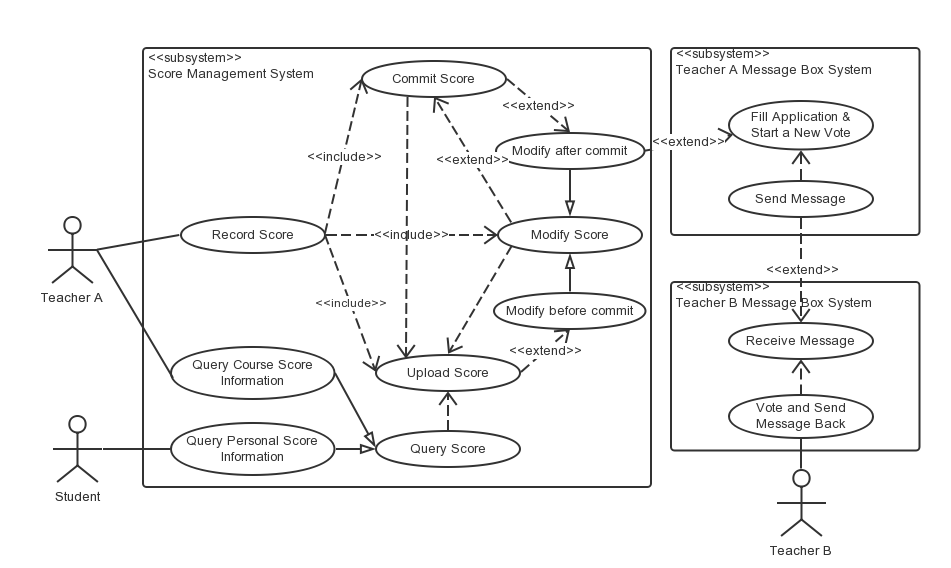
\includegraphics[width=5in]{pic/1.png}
\subsection{Data Flow Diagram}
\subsubsection{Overview}
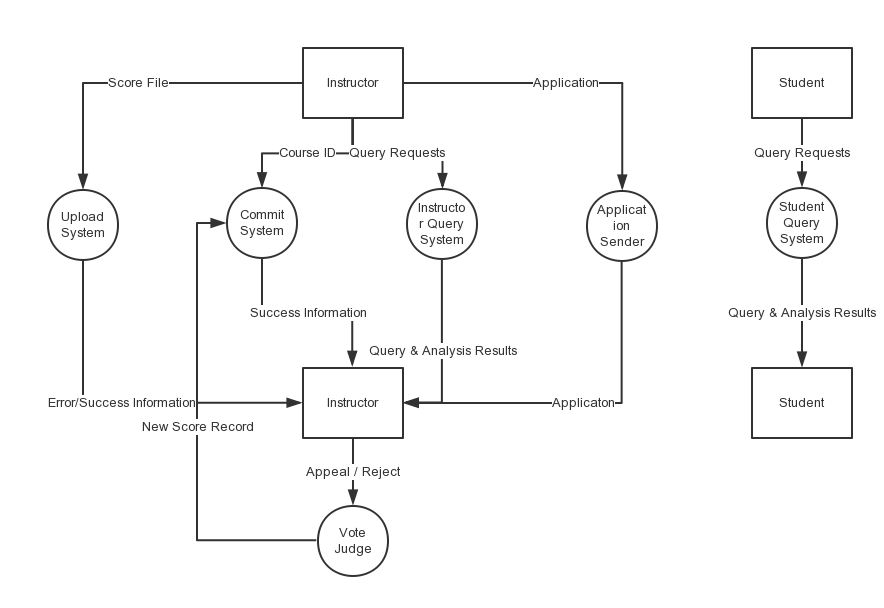
\includegraphics[width=5in]{pic/2-0.png}
\subsubsection{Upload System}
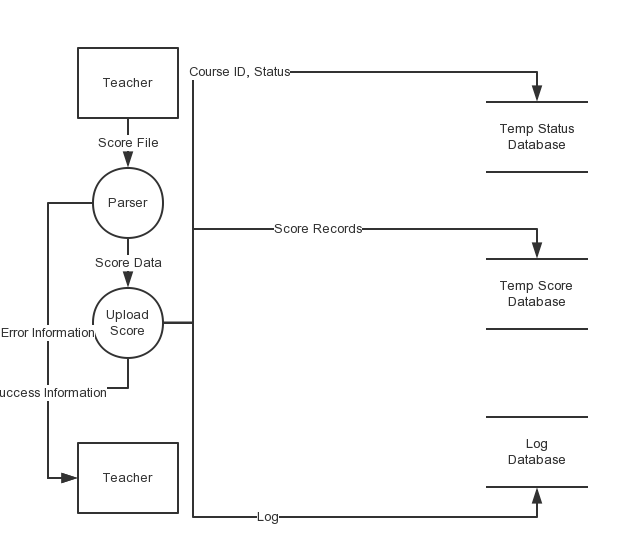
\includegraphics[width=5in]{pic/2-1.png}
\subsubsection{Commit System}
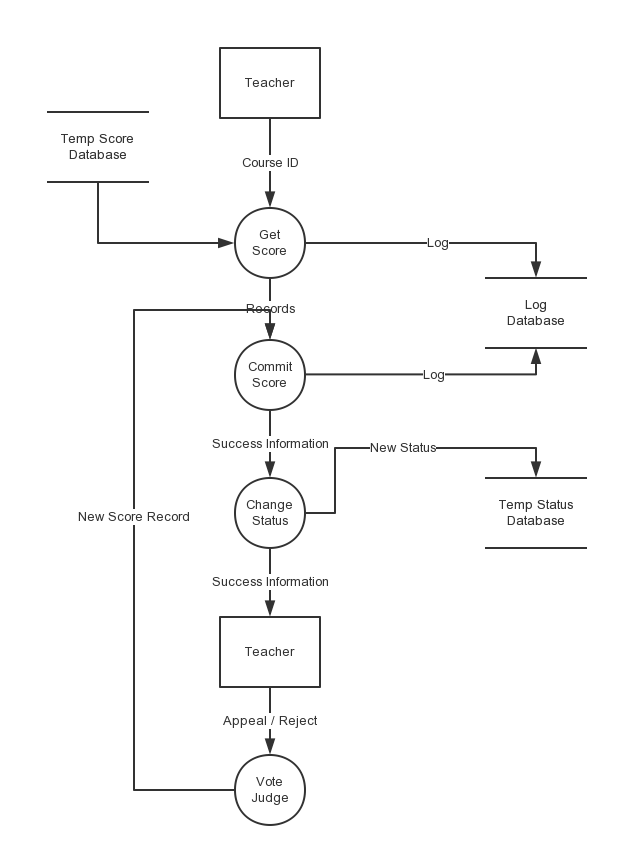
\includegraphics[width=5in]{pic/2-2.png}
\subsubsection{Instructor Query System}
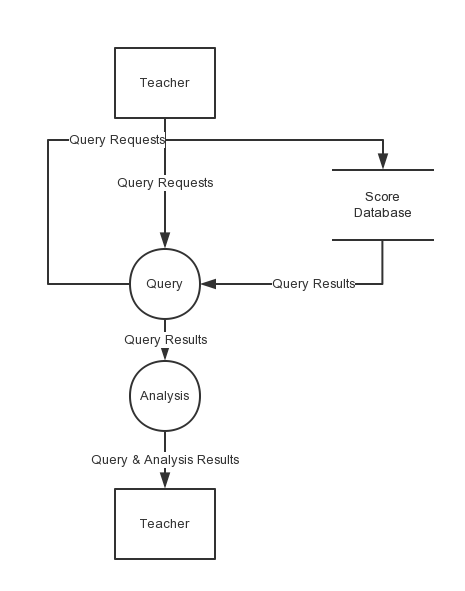
\includegraphics[width=5in]{pic/2-3.png}
\subsubsection{Student Query System}
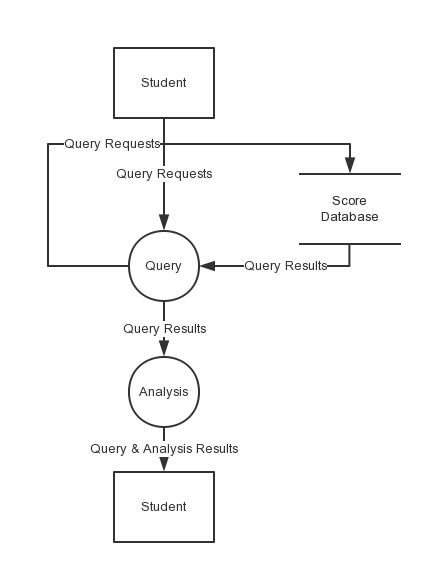
\includegraphics[width=5in]{pic/2-4.png}

\subsection{State Diagrams}
\subsubsection{States Related to Courses}
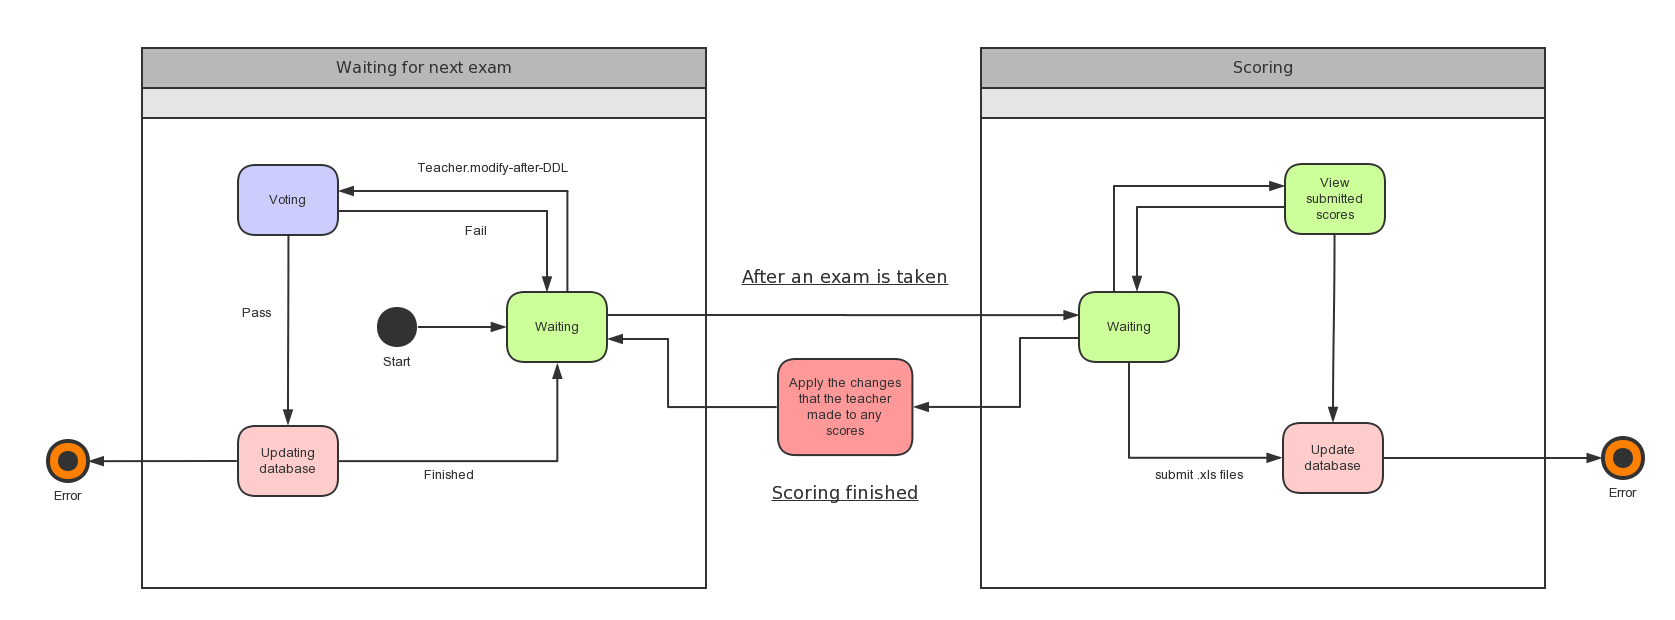
\includegraphics[width=5in]{pic/3-1.png}
\subsubsection{Web State Diagram}
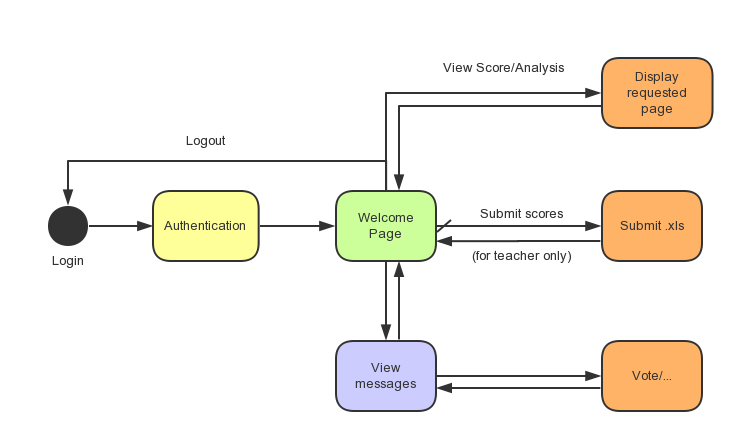
\includegraphics[width=5in]{pic/3-2.png}

\subsection{Class Diagrams}
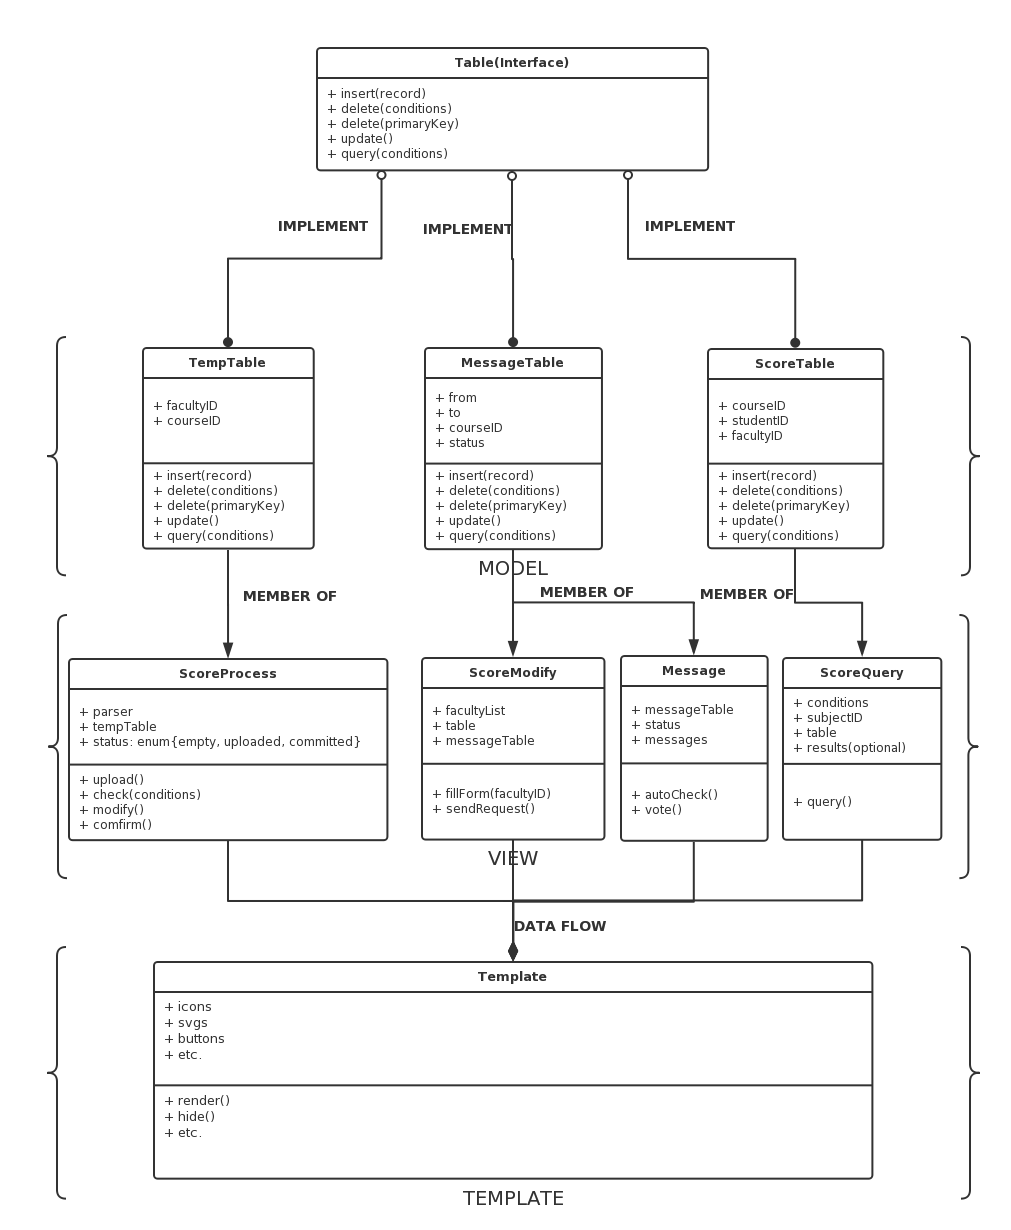
\includegraphics[width=5in]{pic/4.png}
\subsection{CRC Cards}
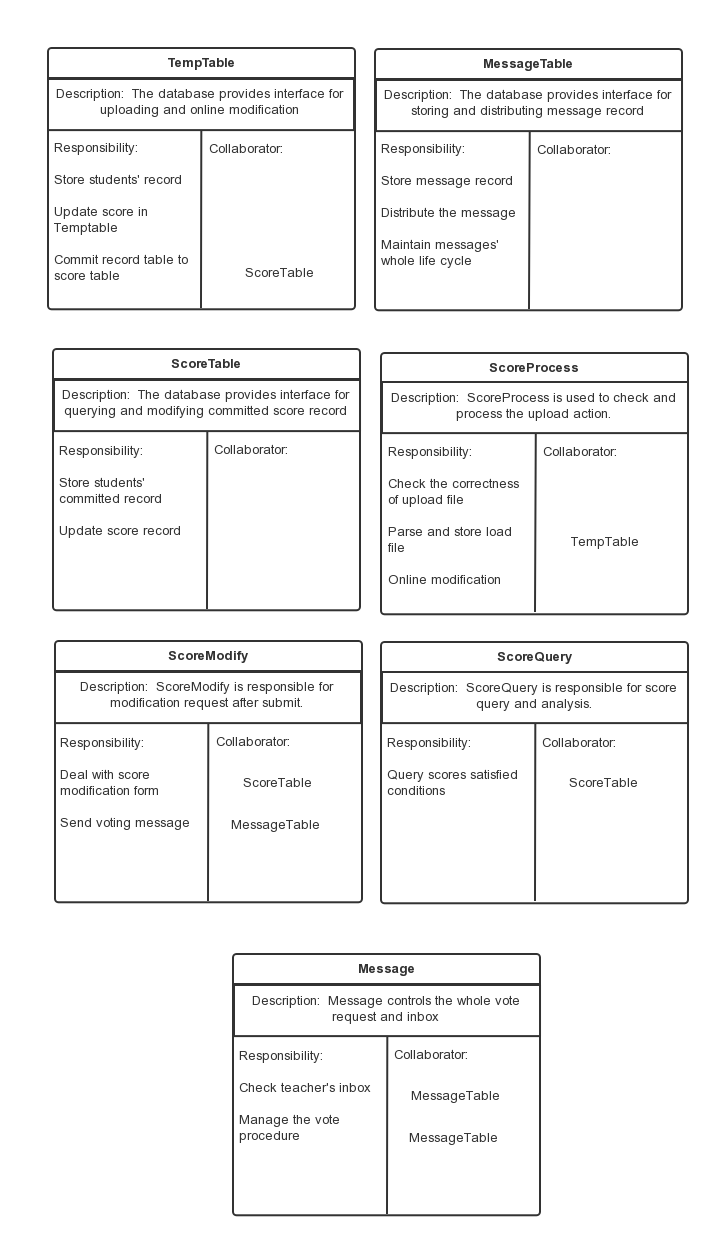
\includegraphics[width=5in]{pic/5.png}
\subsection{Data Description}
\subsubsection{Common}

\begin{itemize}
\item facultyID: the teachers's registered ID

\item courseID: the unique ID of the course lectured at a specific semester by a specific teacher

\item studentID: the student's registered ID

\item score: the number of a student's grade on a specific course.
\end{itemize}


\subsubsection{Message}
the message tool is used to communicate with other users of the system. 
e.g. After the teacher has uploaded the application to modify formally submitted score data, the voting requests will be sent in this message form.
\begin{itemize}
\item from: the sender of the message

\item to: the receiver(s) of the message

\item courseID: the unique ID of the course lectured at a specific semester by a specific teacher

\item status: including several attributes:
\begin{itemize}
\item isPassed: whether this request has passed voting.
\item votedInfo: a array shows that whether all the related teachers have passed, rejected, or haven't read it yet.
\item due date: when will the vote ends.
\end{itemize}
\item send time: when is this message sent.

\end{itemize}










\section{Validation Criteria}

\subsection{Defintion}
\begin{itemize}
\item \emph{Class:} A course instructed by a instructor in a semester.
\item \emph{Relevant Instructor:} The instructor who instructs the same course.
\end{itemize}

\subsection{Functions for Instructors}
\subsubsection{Record Scores}
\begin{enumerate}
\item An instructor could check the information of the classes he/she is currently instructing.
\item An instructor could download a transcript template to be filled from the system.
\item If the format of the transcript meets the criterion, it will be immediately parsed and shown on the screen in tabular form, with class status altered to ``UPLOADED''; otherwise, it will be rejected with detailed reason specified.
\item Any new uploading will directly cover previous files.
\item The scores of the class marked as ``UPLOADED'' could be browsed.
\item The scores of the class marked as ``UPLOADED'' could be directly modified online.
\item Having committed the scores of one class, an instructor could view the statistical information of it, with the class status altered to ``COMMITTED''.
\item The scores of the class marked as ``COMMITTED'' could only be browsed but not be directly modified.
\end{enumerate}

\subsubsection{Vote Modification}
\begin{enumerate}
\item If an instructor wants to modify the scores of a class marked as ``COMMITTED'', he/she needs to fill an online application form including course name, names of students whose scores need modification, new scores and corresponding reasons. All the relevant instructor will be apprised of this request.
\item The relevant instructors can vote for the request for score modification: they could choose either to approve it or to reject it.
\item If all of the relevant instructors agree with this modification, this request will be adopted and the instructor who starts it will get a notification telling the result.
\end{enumerate}
\subsubsection{Query/Analysis Scores}
This is valid after one specific class is marked as ``SUBMITTED''.
\begin{enumerate}
\item The instructor could view score distribution in graphic chart from.
\item The instructor could view ranking statistics in list chart from, including student names, raw scores and grade points.
\item The instructor could view average score in eye-catching place.
\end{enumerate}
\subsection{Functions for Students}
\subsubsection{Query/Analysis Scores}

\begin{enumerate}
\item A student could view score information of all classes that he/she has registered and is marked as ``SUBMITTED''. The score information includes course names, raw scores and grade points.
\item A student could view his/her GPA, average scores, total credits of the current semester.
\item A student could view his/her GPA, average scores, total credits of the courses he/she major in. 

\end{enumerate}

\subsection{Performance}

For score management system, the human interaction inferface is very important. We propose following requirements:
\begin{enumerate}
\item Interface should be simple but specific to functions
\item System should be user friendly and provide help information
\item It should have short response time and provide correctness and efficiency.
\end{enumerate}

\subsection{Security} 
\subsubsection{Privacy} 

Every different User should have own data separated from others. And only owner can access his/her data in System.

\subsubsection{Authentication}

Teachers and students should be detected correctly. Teacher has right to add and update on records, while students don't.

\subsection{Maintenance}

Score manage system can work correctly at most time. And even if it crushes, it can be recovered as soon as possible. Programmer should provide detailed documents and strategies towards every error.


\end{document}


